\section{Aufbau}
Über die Datenbankschnittstelle ließt der Kategorisierer die bislang unkategorisierten Twitteraccounts aus der Accountstabelle. Diese sind durch das Feld \lstinline{Categorized} bestimmt. Dann sucht er in der DMOZ-Datenbank nach passenden Kategorien. Diese werden dann in die Kreuztabelle AccountCategory eingetragen.

Im Diagramm \ref{fig:categorizer} ist der grundlegende Aufbau des Kategorisierers dargestellt:
\begin{figure}[h!]
	\centering
	\includegraphics[width=\textwidth,height=\textheight, keepaspectratio=true]{dia/categorizer}
	\caption{Klassendiagramm des Kategorisierers}
	\label{fig:categorizer}
\end{figure}
\begin{description}
	\item[Account] siehe \cref{sec:datenbankzugriff}
	\item[Category] siehe \cref{sec:datenbankzugriff}
	\item[DBIcategorizer] Über dieses Interface kommuniziert der Kategorsierer mit der Datenbank. Es enthält Methoden zum Holen der unkategorisierten Accounts, zum Finden von Kategorien, zum Eintragen einer Kategorie und zum Auffinden aller Subkategorien einer Kategorie.
	\item[Categorizer] Dies ist die Haupt-Klasse des Kategorisierers. Sie nutzt die Methoden von \lstinline{DBIcategorizer}, um unkategorisierte Accounts zu suchen und gefundene Kategorien einzutragen.
\end{description}

\section{Start des Kategorisierers}
Der Kategorisierer soll in regelmäßigen Abständen vom Betriebssystem gestartet werden und daraufhin die neu gefundenen Accounts kategorisieren.

Der Ablauf des Kategorsierers ist im Sequenzdiagramm \ref{fig:categorizerSeq} zu sehen.
\begin{figure}[h!]
	\centering
	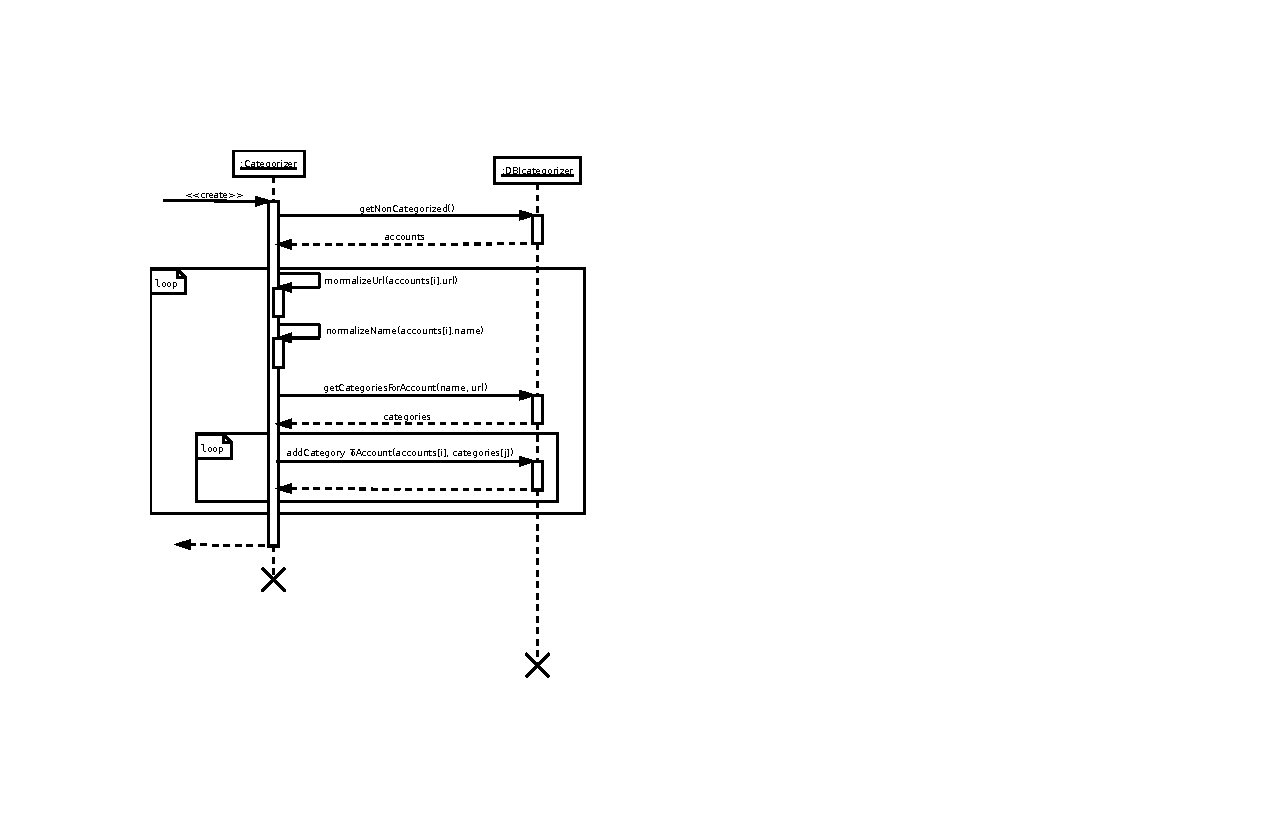
\includegraphics[width=\textwidth,height=\textheight,keepaspectratio=true]{dia/categorizerSequence}
	\caption{Sequenzdiagramm für einen Durchlauf des Kategorisierers. Dabei sind exemplarisch nur jeweils der erste unkategorisierte Account und die erste gefundene Kategorie aufgeführt.}
	\label{fig:categorizerSeq}
\end{figure}

Im ersten Schritt wird also eine Liste von unkategorisierten Accounts ausgelesen. Für jeden dieser Acounts wird eine Liste passender Kategorien ermittelt, die dann nach und nach in die Datenbank geschrieben werden.
